\chapter{Recursion}

\textit{Difficult topic}
\vspace{6mm}

Recursive functions are those which call themselves again inside their function body, for example, the \texttt{fact} function that I will introduce down the chapter.

It might be difficult to get right and understand at first for learners, but it simplifies code once you get used to it. The best way to master it is through looking at more examples. You can see more examples on recursion in the mycodeschool playlist.

\section{Further resources (Ch 4-6)}

Playlists by 
\href{https://www.youtube.com/user/mycodeschool}{mycodeschool}\footnote{Link: \href{https://www.youtube.com/user/mycodeschool}{https://www.youtube.com/user/mycodeschool}}
that focus on 
\href{https://www.youtube.com/playlist?list=PL2\_aWCzGMAwLz3g66WrxFGSXvSsvyfzCO}{recursion}\footnote{Link: \href{https://www.youtube.com/playlist?list=PL2\_aWCzGMAwLz3g66WrxFGSXvSsvyfzCO}{https://www.youtube.com/playlist?list=PL2\_aWCzGMAwLz3g66WrxFGSXvSsvyfzCO}}, 
\href{https://youtube.com/playlist?list=PL2_aWCzGMAwLZp6LMUKI3cc7pgGsasm2_}{pointers}\footnote{Link: \href{https://youtube.com/playlist?list=PL2_aWCzGMAwLZp6LMUKI3cc7pgGsasm2_}{https://youtube.com/playlist?list=PL2\_aWCzGMAwLZp6LMUKI3cc7pgGsasm2\_}} and 
\href{https://www.youtube.com/playlist?list=PL2_aWCzGMAwI3W_JlcBbtYTwiQSsOTa6P}{data structures (linked lists, stacks, queues)}\footnote{Link: \href{https://www.youtube.com/playlist?list=PL2_aWCzGMAwI3W_JlcBbtYTwiQSsOTa6P}{https://www.youtube.com/playlist?list=PL2\_aWCzGMAwI3W\_JlcBbtYTwiQSsOTa6P}}.
mycodeschool explains concepts about computing pretty well. You can also watch his other playlists if interested.

\section{Example: Factorial function}

\begin{lstlisting}
int fact(int x){
    if(x==0) return 1;
    else return x*fact(x-1);
}
//What would happen if we input a negative number?
\end{lstlisting}

Internally, there is a \textbf{call stack}\index{call stack} that stores information about each function call (e.g. the values of the variables, what is left to do) so that they could resume in order.

The figure shows what happens when I call \texttt{fact(4)}

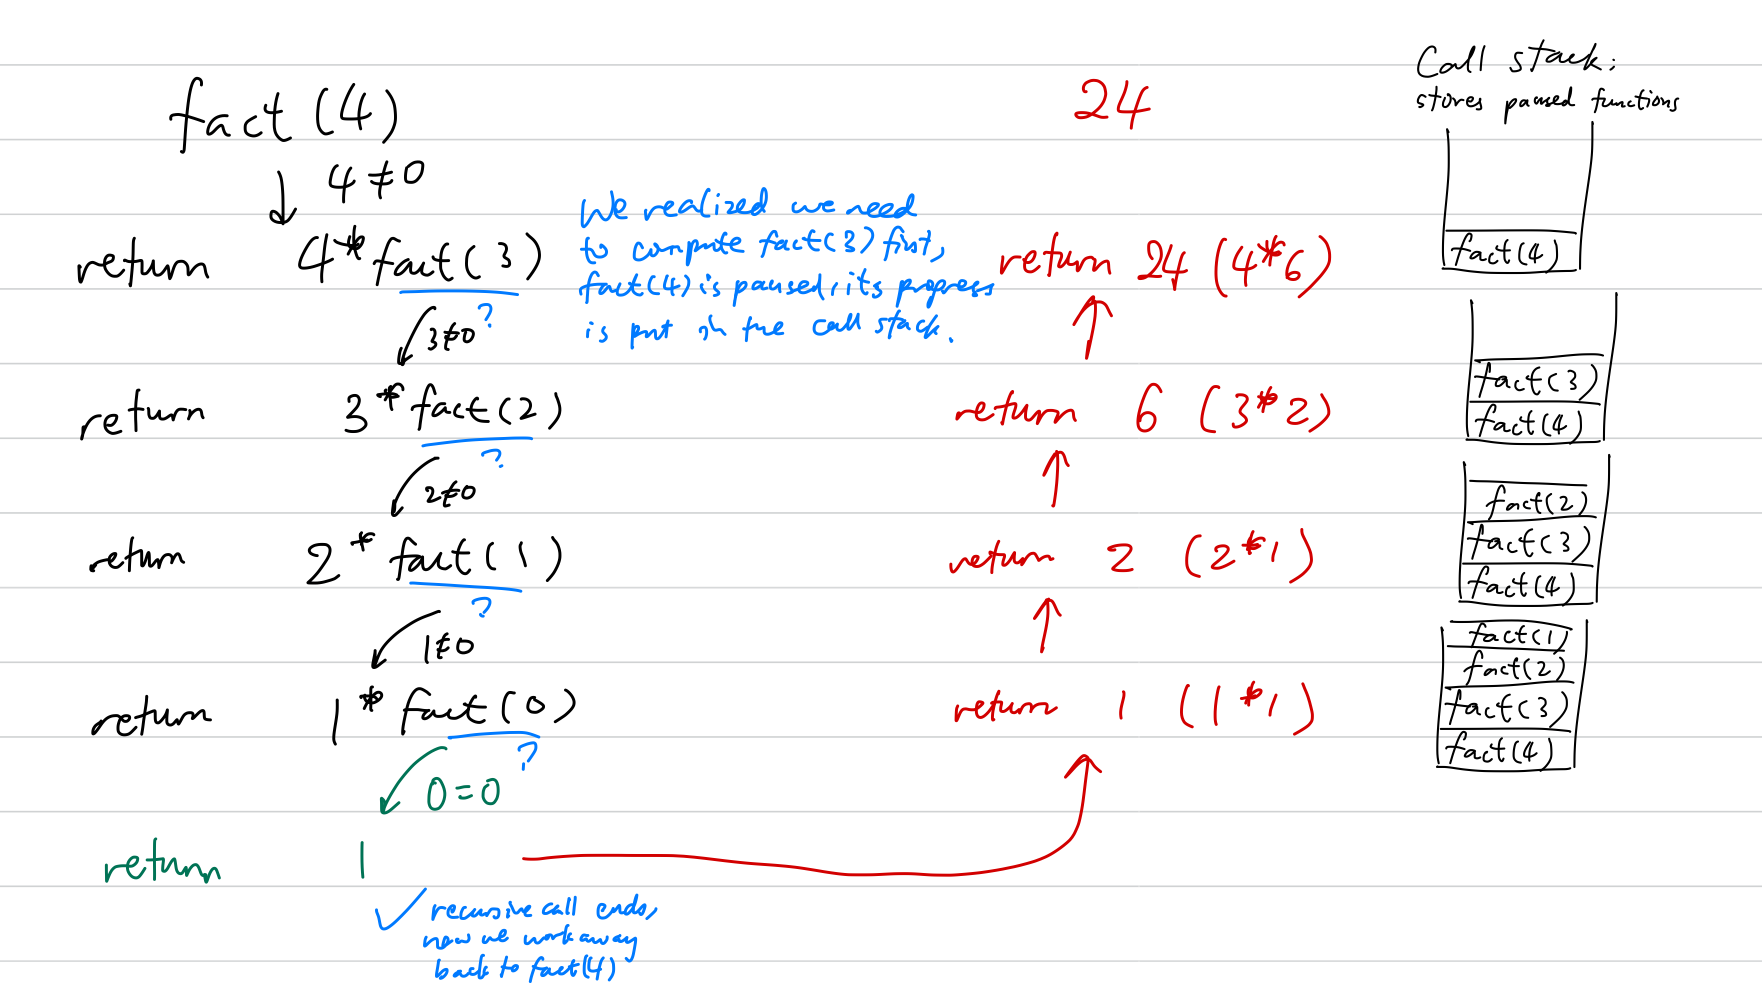
\includegraphics[width=15cm]{ch4-factorial.png}

\texttt{fact(4)} is called, realizing it needs \texttt{fact(3)} to finish, the program pauses \texttt{fact(4)}, and puts it in the call stack, so that it remembers to resume it after getting the result of \texttt{fact(3)}. A similar process happened for \texttt{fact(3)}, \texttt{fact(2)} and \texttt{fact(1)}. Finally, when \texttt{fact(0)} is called, there is no need to rely on other function calls to obtain the return value 1. We call \texttt{fact(0)} the \textbf{base case}\index{base case}. With the result of \texttt{fact(0)}, \texttt{fact(1)} can be resumed, \texttt{fact(1)} is removed from the call stack and its result is computed. A similar process happened for \texttt{fact(2)}, \texttt{fact(3)} and \texttt{fact(4)}, giving the required result finally.

% \section{Example: Fast Exponentiation}
